\documentclass[11pt]{article}
\usepackage[utf8]{inputenc}
\usepackage[T1]{fontenc}
\usepackage{amsmath}
\usepackage{amsfonts}
\usepackage{amssymb}
\usepackage[version=4]{mhchem}
\usepackage{stmaryrd}
\usepackage{graphicx}
\usepackage[export]{adjustbox}
\graphicspath{ {./images/} }

\begin{document}
\section*{Reading}
Forward Contracts on Equities

This section discusses the forward prices set when forward contracts are initiated and when the deliverable or reference asset is a risky asset such as a stock price or an index value. To the extent that the asset underlying the forward contract has systematic risk, the underlying asset will have an expected return that exceeds the riskless interest rate. Financial derivatives on individual equities and equity indices are widely used in alternative investments.

\section*{Determining the Forward Contract Price of a Stock with No Dividends}
This section describes the model for determining the no-arbitrage forward price of risky assets, such as common stocks and stock indices, that pay no dividends. Consider a long position in a growth stock currently valued at $P_{0}$ that will not pay dividends for a long time. Any investor who buys the stock at time 0 at $P_{0}$ receives no dividends but can sell the stock at any time $T$ at its market price, $P_{\mathrm{T}}$. As an alternative strategy an investor can establish a long position in a forward contract on that stock at time 0 for settlement at time $T$. What would be the equilibrium forward price on this stock, $F_{\mathrm{T}}$, for a forward contract initiated at time 0 for settlement at time $T$ ? The answer to this question reveals the essence of forward pricing and lays a foundation on which to build more robust models.

Long positions in forward contracts are commonly and correctly described as financed positions. Financed positions enable economic ownership of an asset without the posting of the purchase price. A long position in a forward contract provides the same economic exposure as a cash position but is obtained without bearing the opportunity cost of funding a cash position. Thus, the key difference between owning the previously mentioned stock versus having a long position in a forward contract on that stock is that the forward position does not require an initial cash outlay (although it may require posting collateral).

A long position in a forward contract held to settlement has only one cash flow, which occurs at time $T$ and is based on the difference between the stock's value at time $T$ and the forward price for the contract on the stock that settles at time $T: P_{T}-F_{T}$. The short side to the forward contract has the same cash flow with the opposite sign: $F_{T}-P_{T}$. Throughout this session, it is assumed that forward contracts are established such that the immediate market value of the contract is zero (i.e., there is no cash payment required from either side to initiate the contract).

Consider an arbitrageur who buys the stock at time 0 and simultaneously establishes a short position in a forward contract to sell the stock at time $T$ for $F_{\mathrm{T}}$. The cash flows to the arbitrageur are $-P_{0}$ at time 0 to buy the stock, $P_{\mathrm{T}}$ from selling the stock at time $T$, and $F_{T}-P_{T}$ at time $T$ from the settlement of the forward contract. Equivalently, the arbitrageur can be viewed as delivering the stock $\left(-P_{T}\right)$ to the long side and receiving the forward price $\left(+F_{T}\right)$ instead of settling the contract with cash $\left(F_{T}-P_{T}\right)$. Since the arbitrageur's short position in the forward contract hedges the risk of the long cash position in the stock, the transaction is riskless and competition will drive the expected return to zero. The net present value (NPV) of the arbitrage is zero and the proceeds at time $T$ are discounted (note that $P_{\mathrm{T}}$ cancels out):


\begin{equation*}
N P V=0=-P_{0}+F_{T} e^{-r T} \tag{1}
\end{equation*}


Note that the subscript to the riskless interest rate has been dropped for expositional simplicity. In all cases where the subscript is dropped, the rate refers to the riskless spot rate with a longevity equal to the time to the respective cash flow or contract settlement. Factoring generates the formula for $F_{T}$-the formula for the forward value in Equation 3 of a financial asset with no dividends or other distributions:


\begin{equation*}
F_{T}=P_{0} e^{r T} \tag{2}
\end{equation*}


\section*{The Forward Contract Price and Accrued Funding Costs}
An important way to conceptualize Equation 2 is that $P_{0} e^{r T}$ is the amount of debt that an arbitrageur (with a short position in a forward contract on the stock) would accrue from borrowing $P_{0}$ dollars at time 0 (to buy the stock), continuously accruing interest on the loan at the rate $r$ and then delivering the stock to the short side of the forward contract at $F_{\mathrm{T}}$. This riskless transaction must have no return in a perfectly competitive market.

Application A starkly illustrates the simplicity of forward pricing by showing that in the case of risky assets with no intervening cash flows (e.g., no dividends), the forward price of the asset is very simply the current market price grossed up for the time value of money rather than being a forecast of the stock's future market value.

\section*{The Forward Price, the Riskless Interest Rate, and Risk Neutrality}
Note that the forward price, $F_{\mathrm{T}}$, in Equation 2 depends on the riskless rate rather than a rate with a risk premium associated with the risk of the equity that underlies the forward contract. The forward price is established at time 0 and in the case of Equation 2 is the risk-neutral future value of $P_{0}$ because it is compounded forward at a riskless rate as if market participants were risk-neutral rather than risk-averse. This use of riskless rates to compound forward risky values at the riskless rate (and to discount risky cash flows at the riskless rate) is central to risk-neutral modeling. The astonishing simplicity of valuation when cash flows can be compounded forward and discounted backward at easily observable riskless interest rates is why financial derivative valuation models are so powerful and derivatives can be such effective risk management tools. Risk-neutral modeling and the resulting valuation models for financial derivatives (e.g., binomial tree models) are key breakthroughs.

Let's examine the intuition of Equation 2. It is only by setting the forward contract price equal to $P_{0} e^{r T}$ at the initiation of the contract that the long position in a forward contract (who bears the risk of fluctuations in the stock) has an expected profit equal to the risk premium of the stock. Because an asset with systematic risk is expected to grow at a rate higher than the riskless rate, the long side of the forward contract in Equation 2 can expect to earn a profit because the forward price uses a lower rate (the riskless rate) to discount future cash flows. Conversely, the short side-who can use the forward contract to lay off the risk of holding the stock -should expect to incur a loss on average from the forward contract because the forward contract transfers the risk of the stock from the entity holding the short position to the entity holding the long position. It therefore makes sense that the forward contract should contain a forward price that offers an expected profit to the long side and an expected loss to the short side.

Another way to view the result is that the only difference, in theory, between the forward contract and cash possession of the stock is that the forward contract is "financed"-it does not require an investment of $P_{0}$ at inception. These "savings" relative to buying the stock now must raise the forward contract price by the riskless rate so that the two can coexist in equilibrium-but not by so much (the risky rate) that there would be no expected profit for bearing the risks of being long a forward contract on a risky asset.

\section*{The Forward Price of a Financial Asset Is an Equality Given the Riskless Interest Rate}
A final important point is that Equation 2 is an equality, not just an inequality. The relationship between the forward price and the spot price was justified by the potential for arbitrage if the relationship did not hold. The discussion of that arbitrage in the section Determining the Forward Contract Price of a Stock with No Dividends described the ability of an arbitrageur to establish a short position in the forward contract and a long position in the underlying asset. This arbitrage makes sure that the forward price is not too high. But the opposite arbitrage approach (establishing a long position in the forward contract and a short position in the underlying asset) will make sure that the forward price is not too low; thus the ability to buy or short sell the underlying asset forces Equation 2 to be an equality.

The exhibit, The Term Structure of Forward Contracts on an Equity Index plots hypothetical forward prices on a non-dividend-paying financial asset against the forward contract's time to delivery (or settlement). The relationship depicted is consistent with Equation 2 and a flat term structure of riskless interest rates. Forward contracts with greater longevity tend to have higher forward prices because the contracts offer the long-side investors exposure to the underlying financial asset at a purchase price that is deferred until delivery. The Term Structure of Forward Contracts on an Equity Index may be viewed as the cumulative savings on funding costs (i.e., the opportunity cost of the capital) by using a forward contract to obtain its underlying asset on a deferred-payment basis rather purchasing the asset in the cash market.

\begin{center}
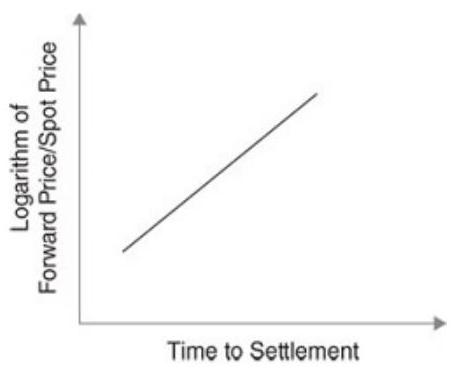
\includegraphics[max width=\textwidth]{2024_04_10_26637806882eb3fbfa51g-03}
\end{center}

The Term Structure of Forward Contracts on an Equity Index

\section*{Determining the Forward Contract Price of a Stock with Dividends}
Let's return to the example of a forward contract on a stock (or stock index) in Application A (within The Forward Contract Price and Accrued Funding Costs section). Recall the forward contract was found to have a $\$ 105.13$ forward price, which was simply found by compounding the stock's current $\$ 100$ value forward for one year at the riskless interest rate of $5 \%$. The result emanated from the perspective of an arbitrageur with a long position in the stock and a short position in the forward contract that generated the following NPV:


\begin{equation*}
N P V=0=-P_{0}+F_{T} e^{-r T} \tag{3}
\end{equation*}


Let's relax the assumption of no dividends in that example by including a non-zero dividend. Specifically, let's assume that the stock will pay a $\$ 3$ dividend with certainty immediately prior to the expiration of the forward contract. The arbitrageur now collects $\$ 3$ extra at time $T$. So the new NPV is:

$$
N P V=0=-P_{0}+F_{T} e^{-r T}-\$ 3 e^{-r T}
$$

$$
F_{T}=P_{0} e^{r T}-\$ 3
$$

Here is the key result: The anticipated dividend of the stock lowers the forward price. A more realistic assumption is to recognize smaller, more frequent dividends. However, the assumption that dividends are paid continuously offers a simple and convenient formula for the forward price of a forward contract on a dividendpaying risky asset such as a stock:


\begin{equation*}
F_{T}=P_{0} e^{(r-q) T} \tag{4}
\end{equation*}


where $q$ is the dividend yield on the forward contract's underlying asset expressed as a continuously paid annual dividend rate. For example, consider the stock with no dividend in Application A (with a riskless rate of 5\%). Let's change the dividend assumption to having the stock distribute a continuous dividend at an annual rate of $3 \%$ (i.e., the stock's annual dividend yield). The forward price would be $\$ 102.02$ using Equation 4.

$$
F_{T}=\$ 100 e^{(.05-.03) \times 1}=\$ 102.02
$$

To the holder of a long position in a forward contract on a dividend-paying stock, the dividend is a cost that drains value out of the stock before the forward contract holder is able to take possession of the stock. Inspection of Equation 4 reveals two key results:

\begin{enumerate}
  \item Higher funding costs to cash positions (i.e., higher riskless rates) make forward contracts more valuable because higher forward contracts are "financed positions." Therefore, the riskless rate enters Equation 4 with a positive sign.

  \item Higher dividend payouts reduce the value of a forward contract by eroding the value of its underlying asset prior to settlement or delivery. Therefore the dividend yield enters Equation 4 with a negative sign.

\end{enumerate}

These two results are why the funding rate (the riskless rate) and the dividend have opposite signs in Equation 4 and will guide the derivation of a formula for a forward price on physical assets in the lesson Forward Contracts on Assets with Benefits and Costs of Carry.

\section*{Four Cases of the Forward Curves of Financial Asset Prices}
The forward prices for financial assets are described in Equation 4. This section expounds on Equation 4 and analyzes the model in four cases with regard to its two parameters: the riskless rate, $r$ (the funding cost), and $q$, the continuous rate of dividends (or other distributions, such as coupons). The forward curve (i.e., the term structure of forward prices) is derived for each case.

Case 1: No Dividends and No Interest: In this simplest case, all forward prices with different delivery dates are equal, and are all equal to the spot price, $P$. This can be verified using Equation 4 with $r=q=0$. The logic of this case is that in the absence of dividends and financing costs, there are no differences between transactions with immediate delivery (spot market) or deferred delivery (forward market). Thus, forward prices must equal spot prices. Thus, any slope or curvature of the forward curve must be driven entirely by dividend rates and financing costs.

The next exhibit illustrates the case of a flat term structure of forward prices, using the horizontal line in the middle of the three structures. The length of time, if any, by which the transaction is deferred (i.e., the time to delivery of the contract) does not change the price at which delivery will take place, since cash pays no interest and the asset pays no dividends. Buyers and sellers are indifferent between immediate exchange and deferred exchange at the same price. The next exhibit also illustrates an upward-sloping and a downward-sloping relationship. In the case of forward contracts on financial securities, the slopes must be related to the cost-ofcarry factors of interest rates and dividends (both of which were assumed to be equal to zero in the previous discussion).

\begin{center}
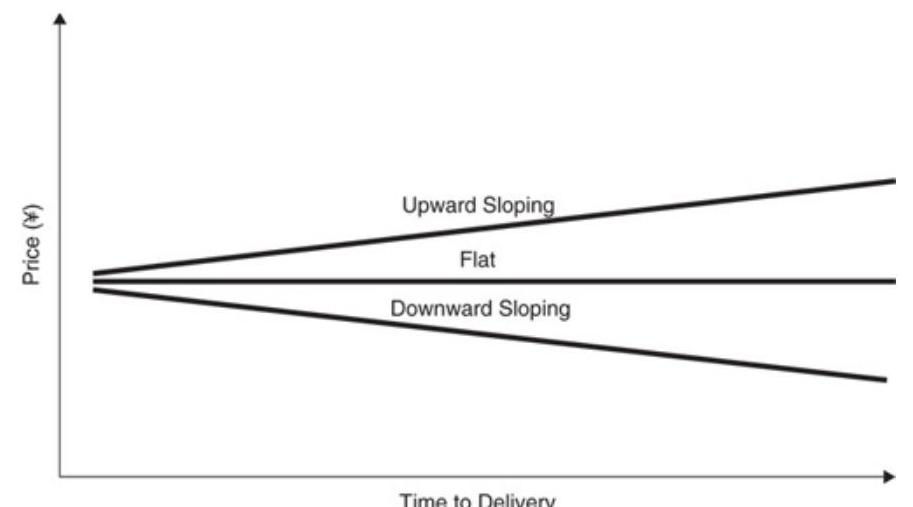
\includegraphics[max width=\textwidth]{2024_04_10_26637806882eb3fbfa51g-04}
\end{center}

\section*{Forward Term Structures}
Case 2: Interest Rates Equal the Dividend Rate: When $r-q=0$, Equation 4 is the same as when both rates are zero. Hence, all the forward prices are equal to the spot price, and the term structure of forward prices is flat. The intuition is that when the benefit of using the spot market (being able to receive dividends) equals the cost of using the spot market (the borrowing cost or opportunity cost of purchasing the asset for cash), the spot and forward prices must be equal.

Case 3: Interest Rates Exceed the Dividend Rate: When $r>q$, then $e^{(r-q) T}>1$, and forward prices will be higher for higher values of $T$. Hence, forward prices are increasing in $T$, and the term structure of forward prices will be upward sloping. Thus, if the spot price of an equity index that pays dividends is $\$ 500$ and if the riskless interest rate exceeds the dividend rate, then every forward contract of every time to delivery will have a forward price equal to $\$ 500 e^{(r-q) T}$, where $(r-q)$ is positive and $e^{(r-q) T}$ is increasing in $T$.

Market participants would be indifferent between (1) using cash to buy the index in the spot market and (2) using forward markets, saving interest ( $r$ ), forgoing dividends $(q)$, and paying a higher price in the forward market than the spot price. The higher forward price than spot price offsets the net gains that forward market participants receive in the form of interest savings that exceed lost dividends.

Case 4: The Dividend Rate Exceeds the Interest Rate: When $r<q$, then $e^{(r-q) T}<1$, and forward prices will be lower for higher values of $T$. With $(r-q)<0, e^{(r-q) T}$ is less than one and decreasing in $T$. The case of $(r-q)<0$ is illustrated in the above exhibit with a downward-sloping forward curve.

An intuitive explanation of why prospective dividends and coupon payments reduce forward prices is that the cash distributions lower the value of a financial asset (i.e., financial asset prices generally fall on days when dividend payments are made). These anticipated declines in spot prices are reflected in the reduction of the prices of forward contracts that call for delivery after the cash distributions.

There is another way to view why forward prices are less than spot prices when $q$ is high and $r$ is low: The value of the deliverable security may be viewed as the sum of the present value of its dividend stream up to time $T$ and the present value of its market price at time $T$. Conceptually, the underlier of a forward contract is only the second term (the present value of the security's future market price). In effect, the inclusion of $q$ in Equation 2 may be viewed as lowering the value of the financial asset to remove the present value of the dividend stream.

In summary, for forward contracts on financial securities, the slope and curvature of the term structure of forward prices (the forward curve) are driven entirely by the relationship between the underlying security's dividend yield and the riskless interest rate (both of which may vary in $T$ ). The forward curve will be flat when $r=q$, upward sloping when $r>q$, and downward sloping when $q>r$. An understanding of these relations serves as an important foundation for understanding many of the issues involved with investing in commodities through futures contracts.


\end{document}